

\tikzset{every picture/.style={line width=0.75pt}} %set default line width to 0.75pt        

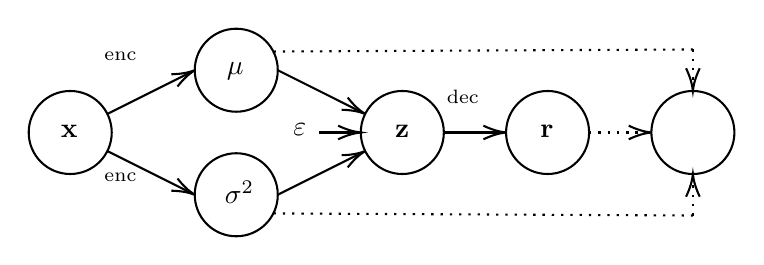
\begin{tikzpicture}[x=0.75pt,y=0.75pt,yscale=-1,xscale=1]
%uncomment if require: \path (0,300); %set diagram left start at 0, and has height of 300

%Straight Lines [id:da7738717285227885] 
\draw    (40,60) -- (98.21,30.89) ;
\draw [shift={(100,30)}, rotate = 513.4300000000001] [color={rgb, 255:red, 0; green, 0; blue, 0 }  ][line width=0.75]    (10.93,-3.29) .. controls (6.95,-1.4) and (3.31,-0.3) .. (0,0) .. controls (3.31,0.3) and (6.95,1.4) .. (10.93,3.29)   ;
%Straight Lines [id:da5615472869000497] 
\draw    (40,60) -- (98.21,89.11) ;
\draw [shift={(100,90)}, rotate = 206.57] [color={rgb, 255:red, 0; green, 0; blue, 0 }  ][line width=0.75]    (10.93,-3.29) .. controls (6.95,-1.4) and (3.31,-0.3) .. (0,0) .. controls (3.31,0.3) and (6.95,1.4) .. (10.93,3.29)   ;
%Straight Lines [id:da4192847666341206] 
\draw    (140,30) -- (180.21,50.11) ;
\draw [shift={(182,51)}, rotate = 206.57] [color={rgb, 255:red, 0; green, 0; blue, 0 }  ][line width=0.75]    (10.93,-3.29) .. controls (6.95,-1.4) and (3.31,-0.3) .. (0,0) .. controls (3.31,0.3) and (6.95,1.4) .. (10.93,3.29)   ;
%Straight Lines [id:da8233466579670681] 
\draw    (140,90) -- (180.21,69.89) ;
\draw [shift={(182,69)}, rotate = 513.4300000000001] [color={rgb, 255:red, 0; green, 0; blue, 0 }  ][line width=0.75]    (10.93,-3.29) .. controls (6.95,-1.4) and (3.31,-0.3) .. (0,0) .. controls (3.31,0.3) and (6.95,1.4) .. (10.93,3.29)   ;
%Straight Lines [id:da3854195120654482] 
\draw    (200,60) -- (248,60) ;
\draw [shift={(250,60)}, rotate = 180] [color={rgb, 255:red, 0; green, 0; blue, 0 }  ][line width=0.75]    (10.93,-3.29) .. controls (6.95,-1.4) and (3.31,-0.3) .. (0,0) .. controls (3.31,0.3) and (6.95,1.4) .. (10.93,3.29)   ;
%Shape: Circle [id:dp5163173181873368] 
\draw  [fill={rgb, 255:red, 255; green, 255; blue, 255 }  ,fill opacity=1 ] (20,60) .. controls (20,48.95) and (28.95,40) .. (40,40) .. controls (51.05,40) and (60,48.95) .. (60,60) .. controls (60,71.05) and (51.05,80) .. (40,80) .. controls (28.95,80) and (20,71.05) .. (20,60) -- cycle ;
%Shape: Circle [id:dp22706934381113864] 
\draw  [fill={rgb, 255:red, 255; green, 255; blue, 255 }  ,fill opacity=1 ] (100,30) .. controls (100,18.95) and (108.95,10) .. (120,10) .. controls (131.05,10) and (140,18.95) .. (140,30) .. controls (140,41.05) and (131.05,50) .. (120,50) .. controls (108.95,50) and (100,41.05) .. (100,30) -- cycle ;
%Shape: Circle [id:dp9715389365150799] 
\draw  [fill={rgb, 255:red, 255; green, 255; blue, 255 }  ,fill opacity=1 ] (100,90) .. controls (100,78.95) and (108.95,70) .. (120,70) .. controls (131.05,70) and (140,78.95) .. (140,90) .. controls (140,101.05) and (131.05,110) .. (120,110) .. controls (108.95,110) and (100,101.05) .. (100,90) -- cycle ;
%Shape: Circle [id:dp38442997347986463] 
\draw  [fill={rgb, 255:red, 255; green, 255; blue, 255 }  ,fill opacity=1 ] (180,60) .. controls (180,48.95) and (188.95,40) .. (200,40) .. controls (211.05,40) and (220,48.95) .. (220,60) .. controls (220,71.05) and (211.05,80) .. (200,80) .. controls (188.95,80) and (180,71.05) .. (180,60) -- cycle ;
%Shape: Circle [id:dp05515800351951605] 
\draw  [fill={rgb, 255:red, 255; green, 255; blue, 255 }  ,fill opacity=1 ] (250,60) .. controls (250,48.95) and (258.95,40) .. (270,40) .. controls (281.05,40) and (290,48.95) .. (290,60) .. controls (290,71.05) and (281.05,80) .. (270,80) .. controls (258.95,80) and (250,71.05) .. (250,60) -- cycle ;
%Straight Lines [id:da41627807567419883] 
\draw    (160,60) -- (178,60) ;
\draw [shift={(180,60)}, rotate = 180] [color={rgb, 255:red, 0; green, 0; blue, 0 }  ][line width=0.75]    (10.93,-3.29) .. controls (6.95,-1.4) and (3.31,-0.3) .. (0,0) .. controls (3.31,0.3) and (6.95,1.4) .. (10.93,3.29)   ;
%Straight Lines [id:da9682561291743264] 
\draw  [dash pattern={on 0.84pt off 2.51pt}]  (290,60) -- (318,60) ;
\draw [shift={(320,60)}, rotate = 180] [color={rgb, 255:red, 0; green, 0; blue, 0 }  ][line width=0.75]    (10.93,-3.29) .. controls (6.95,-1.4) and (3.31,-0.3) .. (0,0) .. controls (3.31,0.3) and (6.95,1.4) .. (10.93,3.29)   ;
%Shape: Circle [id:dp3526949092979663] 
\draw  [fill={rgb, 255:red, 255; green, 255; blue, 255 }  ,fill opacity=1 ] (320,60) .. controls (320,48.95) and (328.95,40) .. (340,40) .. controls (351.05,40) and (360,48.95) .. (360,60) .. controls (360,71.05) and (351.05,80) .. (340,80) .. controls (328.95,80) and (320,71.05) .. (320,60) -- cycle ;
%Straight Lines [id:da60965899132269] 
\draw  [dash pattern={on 0.84pt off 2.51pt}]  (340,100) -- (340,82) ;
\draw [shift={(340,80)}, rotate = 450] [color={rgb, 255:red, 0; green, 0; blue, 0 }  ][line width=0.75]    (10.93,-3.29) .. controls (6.95,-1.4) and (3.31,-0.3) .. (0,0) .. controls (3.31,0.3) and (6.95,1.4) .. (10.93,3.29)   ;
%Straight Lines [id:da10245536402099753] 
\draw  [dash pattern={on 0.84pt off 2.51pt}]  (138,99) -- (340,100) ;
%Straight Lines [id:da1443553940902318] 
\draw  [dash pattern={on 0.84pt off 2.51pt}]  (340,20) -- (340,38) ;
\draw [shift={(340,40)}, rotate = 270] [color={rgb, 255:red, 0; green, 0; blue, 0 }  ][line width=0.75]    (10.93,-3.29) .. controls (6.95,-1.4) and (3.31,-0.3) .. (0,0) .. controls (3.31,0.3) and (6.95,1.4) .. (10.93,3.29)   ;
%Straight Lines [id:da8310403855873987] 
\draw  [dash pattern={on 0.84pt off 2.51pt}]  (138,21) -- (340,20) ;


% Text Node
\draw (34,55) node [anchor=north west][inner sep=0.75pt]    {$\mathbf{x}$};
% Text Node
\draw (55,78) node [anchor=north west][inner sep=0.75pt]    {$\Param_{\mathrm{enc}}$};
% Text Node
\draw (55,20) node [anchor=north west][inner sep=0.75pt]    {$\Param_{\mathrm{enc}}$};
% Text Node
\draw (114,25) node [anchor=north west][inner sep=0.75pt]    {$\mu $};
% Text Node
\draw (113,82) node [anchor=north west][inner sep=0.75pt]    {$\sigma ^{2}$};
% Text Node
\draw (195,55) node [anchor=north west][inner sep=0.75pt]    {$\mathbf{z}$};
% Text Node
\draw (265,55) node [anchor=north west][inner sep=0.75pt]    {$\mathbf{r}$};
% Text Node
\draw (220,38) node [anchor=north west][inner sep=0.75pt]    {$\Param_{\mathrm{dec}}$};
% Text Node
\draw (146,54) node [anchor=north west][inner sep=0.75pt]    {$\boldsymbol{\varepsilon }$};
% Text Node
\draw (333,52) node [anchor=north west][inner sep=0.75pt]    {$\Loss$};


% % Text Node
% \draw (34,55) node [anchor=north west][inner sep=0.75pt]    {$\mathbf{x}$};
% % Text Node
% \draw (66,84) node [anchor=north west][inner sep=0.75pt]    {$\boldsymbol{\phi }$};
% % Text Node
% \draw (66,23) node [anchor=north west][inner sep=0.75pt]    {$\boldsymbol{\phi }$};
% % Text Node
% \draw (114,25) node [anchor=north west][inner sep=0.75pt]    {$\mu $};
% % Text Node
% \draw (113,82) node [anchor=north west][inner sep=0.75pt]    {$\sigma ^{2}$};
% % Text Node
% \draw (195,56) node [anchor=north west][inner sep=0.75pt]    {$\mathbf{z}$};
% % Text Node
% \draw (196,112.4) node [anchor=north west][inner sep=0.75pt]    {$\boldsymbol{\varepsilon }$};
% % Text Node
% \draw (281,52.4) node [anchor=north west][inner sep=0.75pt]    {$\mathbf{x}$};

% % Text Node
% \draw (236,42.4) node [anchor=north west][inner sep=0.75pt]    {$\boldsymbol{\theta }$};


\end{tikzpicture}